\begin{Problem}
	Entscheiden Sie zu jedem der folgenden Objekte, welche der Bezeichnungen aus Definition 2.3.3 darauf zutreffen
	\begin{parts}
		\item $(\R, *,-2)$, wobei $*:\R\times \R\to \R$ durch $a*b:=a+b+2$ definiert ist.
		\item $(\R, \cdot, 1)$
		\item  $\left( \Z / 7\Z, -, 0 \right) $, wobei $\overline{a}-\overline{b}:=\overline{a}+(-\overline{b})$
		\item $\left( \Z \backslash \left\{ 0 \right\} ,*,4 \right) $ mit $*:\Z \backslash \left\{ 0 \right\} \times \Z \backslash \left\{ 0 \right\} \to \Q, (a,b)\to ab^{-1}$
	\end{parts}
\end{Problem}
\begin{proof}
	\begin{parts}
	\item Eine abelsche Gruppe. Es ist assoziativ:
		\begin{align*}
			a*(b*c)=&a+(b+c+2)+2\\
			=&(a+b+2)+c+2\\
			=&(a*b)*c
		\end{align*}
		Es gilt auch $(-2)*x=(-2)+x+2=x $ und auch $x*(-2)=x$ f\"{u}r alle $x$, also $e=-2$ ist ein neutrales Element. F\"{u}r jeder $x$ gibt es auch $y=-(x+4)\in \R$, damit
		\[
		y*x=-(x+4)+x+2=-2=e
		.\] 
	\item Kommutatives Monoid. Per Definition ist $1$ das neutrale Element, und f\"{u}r jeder $0\neq x\in \R$ gibt es $1 / x \in \R$, und $x\left( 1 / x \right) =1$. Aber es existiert keine $x\in \R$, so dass $x 0 = 1$.
	\item Magma. Es gilt
		\begin{align*}
			\overline{a}-(\overline{b}-\overline{c})=&\overline{a}+\left[ -\left(\overline{b}-\overline{c} \right)  \right] \\
			=&\overline{a}+(-\overline{b})+\overline{c}\\
			(\overline{a}-\overline{b})-\overline{c}=&\overline{a}+(-\overline{b})+(-\overline{c})\\
			\neq & \overline{a}-(\overline{b}-\overline{c})
		\end{align*}
		Deswegen ist $-$ nicht assoziativ. 
	\item Nichts. $*$ ist keine Verknüpfung.
	\end{parts}
\end{proof}
\begin{Problem}
	Es sei $(M, \cdot)$ ein Magma, $(H, \circledcirct)$ eine Halbgruppe und $\alpha : H \to M$ eine surjektive Abbildung, die die Bedingung $\alpha\left( a\circledcirct b \right) =\alpha(a)\cdot\alpha(b)$ für alle $a, b \in H$ erfüllt.

	Zeigen Sie
	\begin{parts}
	\item Dann ist auch $M$ eine Halbgruppe.
	\item Ist $H$ ein Monoid mit neutralem Element $e$, dann ist $M$ ein Monoid mit neutralem Element $\alpha(e)$. 
	\item Ist $(H, \circledcirct, e)$ sogar eine Gruppe, dann ist $(M, \cdot, \alpha(e))$ eine Gruppe.
	\end{parts}
\end{Problem}

\begin{proof}
	\begin{parts}
	\item Sei $\beta,\gamma,\delta\in M$. Weil $\alpha$ surjektiv ist, gilt $\beta=\alpha (a), \gamma=\alpha(b), \delta=\alpha(c),a,b,c\in H$. Es gilt
		\begin{align*}
			\beta\cdot(\gamma\cdot\delta)=&\alpha(a)\cdot\left( \alpha(b)\cdot \alpha(c) \right) \\
			=& \alpha(a)\cdot \left( \alpha(b \circledcirct c) \right) \\
			=& \alpha\left( a\circledcirct \left( b\circledcirct c \right)  \right) \\
			=& \alpha\left( \left( a\circledcirct b \right) \circledcirct c \right)\\
			=& \alpha\left( a\circledcirct b \right) \cdot \alpha(c)\\
			=& \left( \alpha(a)\cdot \alpha(b) \right) \cdot \alpha(c)\\
			=& (\beta\cdot\gamma)\cdot\delta
		\end{align*}
	\item Sei $\beta\in M$. Noch einmal haben wir $\beta=\alpha(b), b\in H$. Es gilt
		\begin{align*}
			\beta\cdot \alpha(e)=& \alpha(b)\cdot \alpha(e)\\
			=& \alpha(b\circledcirct e)\\
			=& \alpha(b)\\
			=& \beta
		\end{align*}
		und ähnlich auch für $\alpha(e)\cdot\beta=\beta$.
	\item Wir müssen nur zeigen, dass es ein Inverse gibt. Sei $M\ni \beta=\alpha(a), a\in H$. Weil  $H$ eine Gruppe ist, existiert $a^{-1}\in H$, so dass $a\circledcirct a^{-1}=e$. Es gilt

		 \begin{align*}
			 \beta\cdot \alpha\left( a^{-1} \right) =& \alpha(a)\cdot\alpha\left( a^{-1} \right) \\
			 =& \alpha\left( a\circledcirct a^{-1} \right) \\
			 =& \alpha(e)
		\end{align*}
	\end{parts}
\end{proof}
\begin{Problem}
	Wir wollen die folgende Verkn\"{u}pfungstabelle so vervollst\"{a}ndigen, dass $(\{\partial, \eta, L\}, \circledcirct, \eta)$ zu einer Gruppe wird.
\begin{center}
	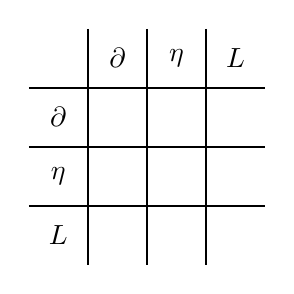
\begin{tikzpicture}[scale=0.75]
		\draw (0,0) node {$\circledcirct$};
		\draw (1,0) node {$\partial$};
		\draw (2,0) node {$\eta$};
		\draw (3,0) node {$L$};
		\draw (0,-1) node {$\partial$};
		\draw (0,-2) node {$\eta$};
		\draw (0,-3) node {$L$};
		\foreach \x in {0,1,2}
		{
		\draw[thick] ({\x+0.5}, 0.5) -- ({\x+0.5}, -3.5);
				\draw[thick] (-0.5,{-\x-0.5}) -- (3.5,{-\x-0.5});
	}
	\end{tikzpicture}
\end{center}
\begin{parts}
\item Begr\"{u}nden Sie, dass es nur h\"{o}chstens eine solche Verkn\"{u}pfungstafel geben kann.
\item F\"{u}llen Sie die Tafel so, dass eine Gruppe entsteht und begr\"{u}nden Sie, dass Sie die Verkn\"{u}pfungs-tafel einer Gruppe gefunden haben.
\end{parts}
\end{Problem}
\begin{proof}
	Notation: Ich schreibe $ab$ statt $a\circledcirct b$, f\"{u}r $a,b\in \left\{ \partial,\eta,L \right\} $. Weil $\eta$ das neutrale Element ist, muss die Verkn\"{u}pfungstabelle so aussehen:	
	\begin{center}
		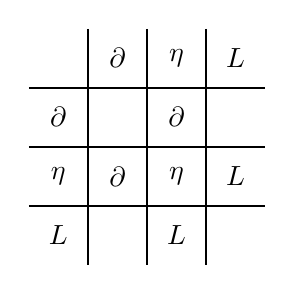
\begin{tikzpicture}[scale=0.75]
			\draw (0,0) node {$\circledcirct$};
			\draw (1,0) node {$\partial$};
			\draw (2,0) node {$\eta$};
			\draw (3,0) node {$L$};
			\draw (0,-1) node {$\partial$};
			\draw (0,-2) node {$\eta$};
			\draw (0,-3) node {$L$};
			\foreach \x in {0,1,2}
			{
				\draw[thick] ({\x+0.5}, 0.5) -- ({\x+0.5}, -3.5);
				\draw[thick] (-0.5,{-\x-0.5}) -- (3.5,{-\x-0.5});
			}
			\draw (2,-1) node {$\partial$};
			\draw (2,-2) node {$\eta$};
			\draw (2,-3) node {$L$};
			\draw (1,-2) node {$\partial$};
			\draw (3,-2) node {$L$};
		\end{tikzpicture}
	\end{center}
Wir brauchen Bedingungen, die mögliche Gruppe einzuschränken.
\begin{Lemma}
	Sei $G$ eine Gruppe, $x,y,z\in G$, und 
	\[
	zx=zy
	.\] 
	Es gilt dann $x=y$
\end{Lemma}
\begin{proof}
	\[
		x=z^{-1}zx=z^{-1}zy=y
	.\] 
\end{proof}
\begin{Corollary}
	In jeder Zeile und Spalte kommt jedes Element nur einmal vor.
\end{Corollary}
Leider ist es noch nicht genug, die Verkn\"{u}pfungstabelle einzuschränken. Wir fangen deswegen an, und nehme an, dass $\partial^2=L$ ist. Wir betrachten die erste Spalte und Zeile, und kommen zu die Schlussfolgerung, dass $\partial L=L\partial=\eta$. 
		\begin{center}
		\begin{tikzpicture}[scale=0.75]
			\draw (0,0) node {$\circledcirct$};
			\draw (1,0) node {$\partial$};
			\draw (2,0) node {$\eta$};
			\draw (3,0) node {$L$};
			\draw (0,-1) node {$\partial$};
			\draw (0,-2) node {$\eta$};
			\draw (0,-3) node {$L$};
			\foreach \x in {0,1,2}
			{
				\draw[thick] ({\x+0.5}, 0.5) -- ({\x+0.5}, -3.5);
				\draw[thick] (-0.5,{-\x-0.5}) -- (3.5,{-\x-0.5});
			}
			\draw (1,-1) node {$\eta$};
			\draw (3,-1) node {$L$};
			\draw (1,-3) node {$L$};
			\draw (2,-1) node {$\partial$};
			\draw (2,-2) node {$\eta$};
			\draw (2,-3) node {$L$};
			\draw (1,-2) node {$\partial$};
			\draw (3,-2) node {$L$};
			\fill[pattern = north east lines] (2.5,-0.5) rectangle (3.5,-3.5);
		\end{tikzpicture}
	\end{center}
Hier gibt es ein Problem: $L\partial = L$, und auch $L\eta=L$. Daraus folgt  $\partial=\eta$, ein Widerspruch. Wir nehmen jetzt an, $\partial^2=L$. Man kann die Verknüpfungstabelle ausfüllen.	
		\begin{center}
		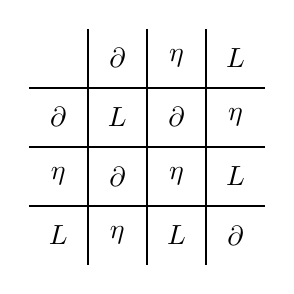
\begin{tikzpicture}[scale=0.75]
			\draw (0,0) node {$\circledcirct$};
			\draw (1,0) node {$\partial$};
			\draw (2,0) node {$\eta$};
			\draw (3,0) node {$L$};
			\draw (0,-1) node {$\partial$};
			\draw (0,-2) node {$\eta$};
			\draw (0,-3) node {$L$};
			\foreach \x in {0,1,2}
			{
				\draw[thick] ({\x+0.5}, 0.5) -- ({\x+0.5}, -3.5);
				\draw[thick] (-0.5,{-\x-0.5}) -- (3.5,{-\x-0.5});
			}
			\draw (2,-1) node {$\partial$};
			\draw (2,-2) node {$\eta$};
			\draw (2,-3) node {$L$};
			\draw (1,-2) node {$\partial$};
			\draw (3,-2) node {$L$};
			\draw (1,-1) node {$L$};
			\draw (3,-1) node {$\eta$};
			\draw (1,-3) node {$\eta$};
			\draw (3,-3) node {$\partial$};
		\end{tikzpicture}
	\end{center}
	Das ist die einzige Lösung (es gibt keine Möglichkeiten mehr). Die Gruppe ist $\cong C_3$. Man kann beachten, dass $\partial^2=L, L^2=\partial$. Per Definition ist es abgeschlossen. Es gilt auch
	\begin{align*}
		\partial^{-1}=&\partial^2=L\\
		L^{-1}=&L^2=\partial
	\end{align*}
	Jetzt beweisen wir Assoziativität. Wir betrachten
	\[
		a(bc)\overset{?}{=}(ab)c,\qquad a,b,c\in \left\{ \partial,\eta,L \right\} 
	.\]
	Im Fall, worin $a,b$ oder $c$ das neutrale Element $\eta$ ist, folgt die Gleichung. Im Fall, worin nichts $\eta$ ist, können wir $L=\partial^2$ einsetzen. Jetzt ist die Gleichung
	\[
	\partial^x\left( \partial^y\partial^z \right) =(\partial^x\partial^y)\partial ^z,\qquad x,y,z\in \left\{ 1,2 \right\} 
	,\] 
	was immer gilt, weil die beide Seite gleich $\partial^{x+y+z}$ sind. Deswegen ist $\circledcirct$ assoziativ.
\end{proof}

\begin{Problem}
	Wir definieren die drei Abbildungen $c_1, c_2, c_3 : \{1, 2, 3, 4\} \to \{1, 2, 3, 4\}$ durch die Abbildungsvorschriften
	\begin{align*}
	& 	c_1(1)=2 & c_1(2) = 1 & & c_1(3) = 4 & & c_1(4)=3\\
	& c_2(1)=3 & c_2(2)=4 & & c_2(3) = 1 & & c_2(4)=2 \\
	& c_3(1) = 4 & c_3(2) = 3 & & c_3(3) = 2 & & c_3(4) = 1
	\end{align*}
	Zeigen Sie: $U := \{\text{id}, c_1, c_2, c_3\}$ ist eine Untergruppe von $S(\{1, 2, 3, 4\})$.
\end{Problem}
\begin{proof}
	Die folgende Aussagen können durch direkte Verkettung bewiesen werden:
	\begin{align*}
		c_1\circ c_2=&c_3\\
		c_2\circ c_3=&c_1\\
		c_3\circ c_1=&c_2\\
		c_1\circ c_1=&\text{id}\\
		c_2\circ c_2=&\text{id}\\
		c_3\circ c_3=&\text{id}
	\end{align*}
	Deswegen ist jede Elemente invertierbar. Es folgt daraus auch, dass $U$ abgeschlossen ist. $\text{id}$ ist natürlich das neutrale Element.
\end{proof}
\begin{Problem}
	Es sei
	\[
		\mathcal{L}:=\left\{ f:\R\to\R|\text{ ex existieren }a,b\in \R, a\neq 0, \text{ sodass f\"{u}r alle }x\in \R f(x)=ax+b \right\} 
	.\] 
	\begin{parts}
	\item Zeigen Sie: $\left( \mathcal{L},\circ, \text{id} \right) $ ist eine Gruppe, aber nicht abelsch.
	\item Wir definieren die Relation $\sim\subseteq \mathcal{L}\times \mathcal{L}$ durch die Festlegung $f\sim g$ genau dann, wenn $f(x)-f(0)=g(x)-g(0)$ f\"{u}r alle $x\in \R$ gilt.

		Zeigen Sie, dass dies eine Äquivalenzrelation ist und bestimmen Sie die Menge aller Äquivalenzklassen von $\sim$.
	\end{parts}
\end{Problem}
\begin{proof}
	\begin{parts}
	\item Sei $f,g\in \mathcal{L}$, $f=ax+b, g=cx+d, a\neq 0 \neq c$. Es gilt
		 \begin{align*}
			 (f\circ g)(x)=&a(cx+d)+b\\
			 =&acx+ad+b
		\end{align*}
		Weil $a\neq 0 \neq 0$, gilt $ac\neq 0$. Deswegen gilt, f\"{u}r
		\[
		h:\R\to \R, h(x)=acx+ad+b
		\]
		$h\in \mathcal{L}$. $(\mathcal{L},\circ,\text{id})$ ist dann unter $\circ$ abgeschlossen. Die Verkettung von Abbildungen ist immer assoziativ. Sei jetzt $e\in \mathcal{L}$, $e(x)=1x+0=x$. Es gilt dann
		\[
		e\circ f = f\circ e=f
		,\]
		also $e$ ist ein neutrales Element. Sei $f^{-1}:\R\to \R$, $f^{-1}(x)=\frac{1}{a}x-\frac{b}{a}$. Weil $a\neq 0$, sind $1 / a$ und $b / a$ wohldefiniert, und $1 / a\neq 0$. Es gilt
		\begin{align*}
			(f\circ f^{-1})(x)=& a\left( \frac{x}{a}-\frac{b}{a} \right) +b\\
			=& x-b+b\\
			=&x\\
			\left( f^{-1}\circ f \right) =& \frac{1}{a}\left( ax+b \right) -\frac{b}{a}\\
			=& x+\frac{b}{a}-\frac{b}{a}\\
			=&x
		\end{align*}
		Deswegen gilt $f\circ f^{-1}=e=f^{-1}\circ f$, also $f^{-1}$ ist die Inverse von $f$. $\mathcal{L}$ ist dann eine Gruppe.
	\item 
		\begin{enumerate}[label=(\roman*)]
			\item (Reflexivität) Es gilt
				\[
				f(x)-f\left(0 \right) =f(x)-f(0)
				\]
				f\"{u}r alle $x\in \R$.
			\item (Symmetrie) Falls gilt
				\[
				f(x)-f(0)=g(x)-g(0)
				\]
				f\"{u}r alle $x\in \R$, gilt auch
				 \[
				g(x)-g(0)-f(x)-f(0), x\in \R
				.\] 
			\item (Transitivität) Sei $f,g,h\in \mathcal{L}$, f\"{u}r die gilt
				\begin{gather*}
					f\sim g \iff f(x)-f(0)=g(x)-g(0), x\in \R\\
					g\sim h \iff g(x)-g(0)=h(x)-h(0), x\in \R
				\end{gather*}
				Es gilt, von die Transitivät der $=\subseteq \R\to \R$, dass
				\[
				f(x)-f(0)=h(x)-h(0), x\in \R
				,\]
				also $f\sim h$
		\end{enumerate}
		Ich vermute, dass die Äquivalenzklasse sind $f,g\in \mathcal{L},f(x)=ax+b,g(x)=cx+d,a\neq 0 \neq c$, so dass
		\[
		f\sim g \iff a = c
		.\]
		Wir beweisen es: $f(0)=b, g(0)=d$, und daher $f(x)-f(0)-ax, g(x)-g(0)=cx$. Falls
		\[
		ax=cx\forall x\in \R
		,\]
		muss $a=c$.  F\"{u}r $a\neq c$ gilt es, dass es mindestens ein Punkt $x_0\in \R$ gibt, worauf $ax_0\neq cx_0$. Deswegen sind die Äquivalenzklassen, f\"{u}r $f,g\in \mathcal{L}$, $f=ax+b,g=cx+d$
		 \[
		f\sim g \iff a = c
		.\qedhere\] 
	\end{parts}
\end{proof}
